\section{CREATION} 
Elle a été créée en 2009 par 2 ingénieurs ayant travaillés pendant plus de 10 ans pour les grands intégrateurs français et sur de nombreux comptes clients. La Sarl INSBI (Institut Business Intelligence) a une ligne directrice essentiellement centrée sur l’informatique décisionnel (Business Intelligence). Elle travaille avec une dizaine de collaborateurs en réseaux. 
En 2013, Sarl INSBI s’associe à la SAS IFICLIDE et prend la direction et le développement du pôle business intelligence. Depuis le début d’année 2017, l’associé Rodrigue Kendjio a entrepris l’extension des activités en Afrique. Amorcé dès le second trimestre 2017 par un projet d’e-commerce, le lancement officiel des activités est prévu au Cameroun à la fin d’année 2017.

2.	MISSION :
Là où le contexte est en évolution permanente et les facteurs majeurs de transformation sont centrés sur les défis concurrentiels et la globalisation de l’information, nos experts interviennent pour vous accompagner dans la mise en place de projets informatiques : d’INFRASTRUCTURES, D’APPLICATIONS et de services.
Nous intervenons dans le domaine bancaire, l’assurance la grande distribution et l’industrie

\section{PRESENTATION}
\textbf{Conseil}
	\begin{list}{•}{ }
	 \item Stratégique : Accompagner les directions générales dans leur besoin de pilotage
	\item Métier : Guider les directions métiers dans l’expression de leurs besoins
	\item Technologique : Aider au choix de solution de gestion et d’aide à la décision
	\item Conduite du changement : Faciliter, valoriser et promouvoir le changement
	\end{list}
\section{Réalisation}
\begin{list}{•}{ }
   \item Audit : Analyser l’existant et réaliser l’étude d’impact
	\item Gestion de projet : Piloter et animer le projet
	\item Technique : Concevoir et mettre en œuvre le système d’information BI
   \item Formation : Former les utilisateurs à la nouvelle plateforme
\end{list}

\section{Exploitation}

\begin{figure}[h]
	\begin{center}
		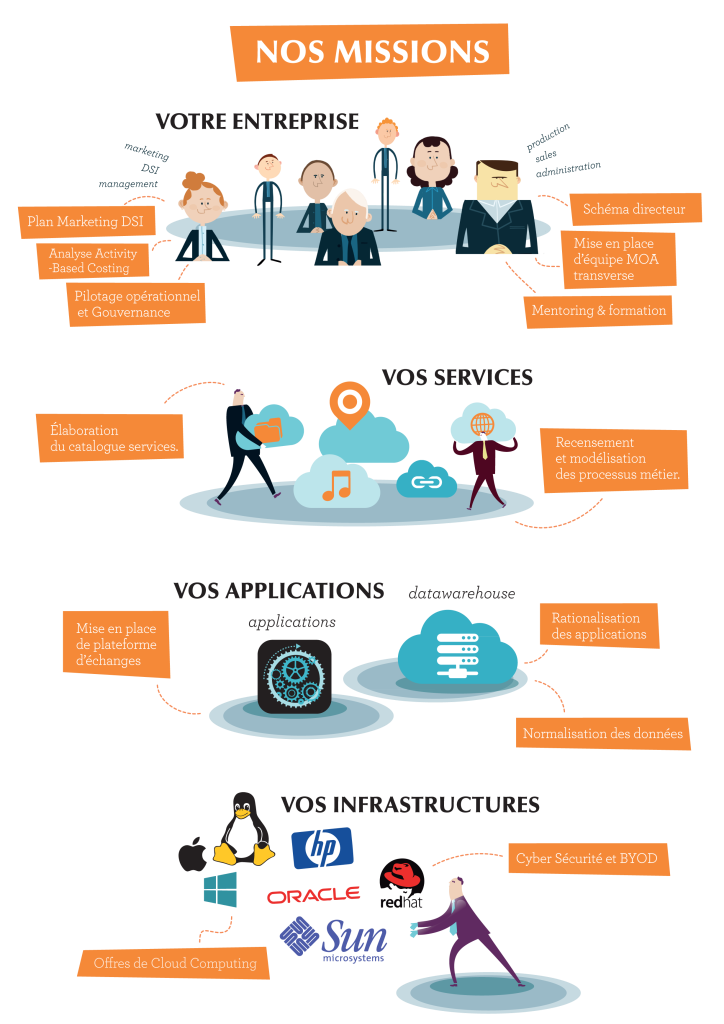
\includegraphics[scale=0.75]{images/missions.png}
		\caption{Présentation de INSBI}
		\label{presentation}
	\end{center}
\end{figure}

\cleardoublepage
\section{CLIENTS}
   \begin{list}{•}{ }
   \item Oracle,
   \item Easyteam (SEDIF, APRIA RSA),
   \item Logica (PROBTP, MMPJ)
   \item Smarthys (AUTOLIV)
   \item TECHNIP  Flexi France
   \item Société Générale
   \end{list}

\begin{figure}[h]
	\begin{center}
		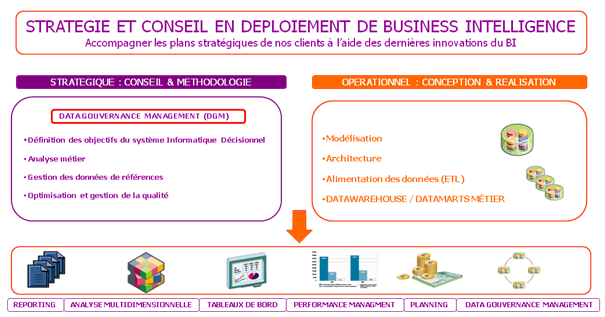
\includegraphics[scale=0.85]{images/deuxieme.png}
		\caption{Activité de INSBI}
		\label{synthese-cout-salarie}
	\end{center}
\end{figure}










